\section{Analysis: PCF  and Gap-Junction Response to Constant Stimulus}

 We compare the network estimate of all three models (PCF, gap-junction, and self-coupled) for the case of a constant driving stimulus. 
 
 Let all 3 models have the same parameters as given by equation (\ref{eq:analysis:comparison_sc_vs_pcf_vs_gj:pcf_demo_sim_params}) with the exception that 

\begin{align*}
	c(\xi) &= c = 
	\begin{bmatrix}
		1 \\ 0	
	\end{bmatrix}, 
\end{align*}
and
$x(0) = \begin{bmatrix} \frac{1}{2} & 0 \end{bmatrix}$. 
 
 \subsection{PCF Network Response to Constant Stimulus:}

From equation (\ref{eq:analysis:comparison_sc_vs_pcf_vs_gj:pcf_voltage_dynamics}), the PCF dynamics become
\begin{align*}
	\dot{V}_{pcf}
	&=
	- V_{pcf}
	+
	D^T 
	\left(
		-I + I
	\right)
	D^T r
	+
	D^T 
	\begin{bmatrix}
		1 \\ 0
	\end{bmatrix}
	-
	D^T D o
	%
	\\
	\\
	%
	&= 
	-V_{pcf}
	+ 
	D^T 
	\begin{bmatrix}
		1 \\ 0
	\end{bmatrix}
	-
	D^T D o.
\end{align*}
All voltages are initially 0. From equation (\ref{eq:analysis:comparison_sc_vs_pcf_vs_gj:pcf_spiking_behavior}) the thresholds are identically $\frac{1}{2}$. Until the first spike, neuron $j$'s voltage integrates the quantity $d_j^T 	\begin{bmatrix}	1 \\ 0	\end{bmatrix}$. Denote the neuron $j$ whose tuning curve $d_j$ is closest in angle to $c$ by 

\begin{align*}
	j_{max} \overset{\Delta}{=}
	 \underset{
	 	i \in 
	 	\left[
	 		1, \ldots, N
	 	\right]
	 }
	 {argmax}
	 \hspace{4mm}
	 	d_j^T c.
\end{align*}
Neuron $j_{max}$ will receive the highest driving force and will therefore reach its threshold  before any other neuron. It will then be reset by $1$ to $- \frac{1}{2}$. Each other neuron $k$ will also be reset (decremented) by $d_k^T d_{j_{max}}$, proportional to their angle relative to both neuron $j_{max}$ and the driving strength $c$. This sequence will repeat periodically so that only neuron $j_{max}$ fires at a constant rate. 

We write the PCF network as the one-dimensional equation

\begin{align*}
	v_{pcf} &= 
	- v_{pcf}
	+ d_{j_{max}}^T c 
	- o_{j_{max}}.
\end{align*}

This is a form of the leaky integrate-and-fire (LIF) model, with drive term $d_j^T c(\xi)$. The neuron is driven by inner product $d_{j_{max}}^T c$. Note from equation (\ref{eq:analysis:comparison_sc_vs_pcf_vs_gj:pcf_spiking_behavior}) that the threshold voltage varies with $||d_{j_{max}}||^2$.  For clarity, we drop the subscripts $j$, $j_{max}$ in the following equations. It is understood that we are referring to the solely spiking neuron $j_{max}$.
With initial condition $v_{pcf}(0) = - \frac{||d||^2}{2}$, the neuron's trajectory is integrated as 
\begin{align}
\label{eq:analysis:comparison_sc_vs_pcf_vs_gj:const_stim:pcf_voltage_trajectory}
	v_{pcf}(\xi)
	&= 
	d^T c - e^{-\xi} 
	\left(
		d^T c + \frac{||d||^2}{2}
	\right). 
\end{align}

The neuron spikes when it reaches the threshold $v_{pcf} = ||d||^2$. To compare with the self-coupled network, we note that the singular value associated with neuron $j$ of the decoder matrix $S = ||d||^2$.

From the preceding equation with voltage at  threshold $\frac{||d||^2}{2}$,
\begin{align*}
	\frac{||d||^2}{2}
	&= 
	d^T c - e^{-\xi_{spike}} 
	\left(
		d^T c + \frac{||d||^2}{2}
	\right)
	%
	\\
	\\
	%
	\implies
	e^{-\xi_{spike}}
	&= 
		\frac
	{
		d^T c - \frac{||d||^2}{2}
	}
	{
		d^T c + \frac{||d||^2}{2}
	}
	%
	\\
	\\
	%
	\implies
	\xi_{spike}
	&= 
	ln
	\left(
		d^T c + \frac{||d||^2}{2}
	\right)
	-
	ln
	\left(
		d^T c - \frac{||d||^2}{2}
	\right)		
\end{align*}
This leads to a firing rate 

\begin{align}
\label{eq:analysis:comparison_sc_vs_pcf_vs_gj:const_dynamics:pcf_spike_rate}
	\phi_{pcf}
	\left(
		d
	\right)
	 =
	 \frac
	 {
	 	1
	 }
	 {
		ln
		\left(
			d^T c + \frac{||d||^2}{2}
		\right)
		-
		ln
		\left(
			d^T c - \frac{||d||^2}{2}
		\right)		
	}
\end{align}

Deriving the network estimate, suppose it begins at $x(0)$. The trajectory until the first spike at time $\xi_1$ is
$$
\hat{x}(\xi) = x(0) e^{-\xi}, \hspace{4mm} 0 \leq \xi < \xi_1.
$$

The spike adds $d$ to the readout followed by exponential decay:
$$
\hat{x}(\xi) =
\left(
	x(0) e^{-\xi_1}
    +
	d
\right)
 e^{-(\xi-\xi_1)} , \hspace{4mm} 0 \leq \xi-\xi_1 < \frac{1}{\phi}.
$$
Until the third spike the readout is
$$
\hat{x}(\xi) =
\left(
	x(0) e^{-\xi_1} e^{-\frac{1}{\phi} }
    +
	d e^{-\frac{1}{\phi}}
	+ d
\right)
 e^{-(\xi - \frac{1}{\phi} - \xi_1)}
	 , \hspace{4mm} \frac{1}{\phi} \leq \xi-\xi_1 < \frac{2}{\phi}.
$$
The recursive pattern is visible after the third spike
$$
\hat{x}(\xi) =
\left(
	x(0) e^{-\xi_1} e^{-\frac{2}{\phi} }
    +
	d e^{-\frac{2}{\phi}}
	+ d e^{-\frac{1}{\phi}}
	+d
\right)
 e^{-(\xi - \frac{2}{\phi} - \xi_1)}
	 , \hspace{4mm} \frac{2}{\phi} \leq \xi-\xi_1 < \frac{3}{\phi}.
$$

Consider the $n^{th}$ term for $n$ big enough so that the $x(0)$ term is approximately $0$. The readout at spike time $\xi_n$ is given by the sum
$$
\hat{x}(\xi_n) =  d \sum_{l = 0}^{n-1} e^{-\frac{l}{\phi}}.
$$
The series converges to 
$$
\hat{x}(\xi_n) =  
\frac
{
	d
}
{
	1 - e^{-\frac{1}{\phi}}.
}
$$
Between the spikes the readout exponentially decays so that the network estimate is given by

\begin{align}
\label{eq:analysis:comparison_sc_vs_pcf_vs_gj:const_dynamics:pcf_network_estimate_steady_state}
\hat{x}_{pcf}(\xi) =
\frac
{
	d
}
{
	1 - e^{-\frac{1}{\phi}}
}
e^
{
	- \hspace{2mm}
	\left(
		\xi - \xi_1^1
	\right)
	\mod
	{
		\frac
		{
			1
		}
		{
			\phi
		}
	}
}.
\end{align}


\subsection{Gap-Junction Network Response to Constant Stimulus:} Here we derive the decoded estimate of a gap-junction network driven by a constant stimulus, $c(\xi) = \begin{bmatrix}
1 & 0
\end{bmatrix}
$. All other parameters are identical to those in equation (\ref{eq:analysis:comparison_sc_vs_pcf_vs_gj:pcf_demo_sim_params}).

From the dynamics equation (\ref{eq:analysis:comparison_sc_vs_pcf_vs_gj:gj_voltage_dynamics}) gap-junction voltages are continuously coupled to one another via $D^T A D^{T \dagger}$. We thus need to solve the entire system between spikes rather than reducing it to a single dimension. Let $\tilde{[]}$ denote the Laplace transform of a variable. Assume neuron j has just spiked so that 

\begin{align*}
V(0) = -\frac{1}{2}
\begin{bmatrix}
d_1 ^T d_j
\\
\vdots
\\
d_j^T d_j
\\
\vdots
\\
d_N^T d_j
\end{bmatrix}.
\end{align*}

Since $c(\xi) = \begin{bmatrix}
1 \\ 0
\end{bmatrix}$, $B = I$, and $o(\xi) = 0$ between spikes, we have

$$
	\dot{V} 
	=
	D^T A D^{T \dagger} V
	+ 
	D^T 
	\left(
		A + I
	\right)
	D r
	+
	d_1,
$$
where $d_1$ is the first column of $D$. 
Apply the one-sided Laplace Transform to both sides and use the Laplace derivative property:
\begin{align*}
	s \tilde{V} - V(0)
	&=
	D^T A D^{T \dagger} \tilde{V}
	+
	D^T 
	\left(
		A + I
	\right)o
	D \tilde{r}
	+
	\mathcal{L}\left[d_1\right]
	%
	\\
	\\
	%
	\implies
	\left(
	s \, I - D^T A D^{T \dagger} 
	\right)
	\tilde{V}
	&=
	V(0)
	+
		D^T 
	\left(
		A + I
	\right)
	D \tilde{r}
	+
	\tilde{d_1}	
	%
	\\
	\\
	%
	\implies 
	\tilde{V}
	&= 
	\left(
	s \, I - D^T A D^{T \dagger} 
	\right)^{-1}
	\left[
		V(0)
		+
		D^T 
		\left(
			A + I
		\right)
		D \tilde{r}
		+
		\tilde{d_1}	
	\right]
	%
	\\
	\\
	%
	&= 
	\left(
		sI - D^T A D^{T \dagger}
	\right)^{-1}
	V(0)
	+ 
		\left(
		sI - D^T A D^{T \dagger}
	\right)^{-1}
	D^T 
	\left(
		A + I
	\right)	
	D \tilde{r}
	+
	\tilde(d_1).
\end{align*}

Now apply the inverse Laplace transform. Note that by definition of matrix exponential, 

$$
	\mathcal{L}^{-1} 
	\left(
		sI - D^T A D^{T \dagger}
	\right)^{-1}
	= e^{\xi D^T A D^{T \dagger}}.
$$
Therefore, 
\begin{multline}
\label{eq:analysis:comparison_sc_vs_pcf_vs_gj:gj_voltage_intermittent_laplace_transformed}
	V(\xi)
	=
	e^{\xi D^T A D^{T \dagger}} V(0)
	+
	\mathcal{L}^{-1}
	\left[
		\left(
			sI - D^T A D^{T \dagger}
		\right)^{-1}
		D^T B \tilde{c}
	\right]
	\\
		+ 
	\mathcal{L}^{-1}
	\left[
		\left(
			sI - D^T A D^{T \dagger}
		\right)^{-1}
		D^T 
		\left(
			A + I
		\right)	
		D \tilde{r}
	\right].
\end{multline}
\\
To simplify the second term of equation (\ref{eq:analysis:comparison_sc_vs_pcf_vs_gj:gj_voltage_intermittent_laplace_transformed}), use the convolution-product property of the Laplace transform to get
\\
$$
	\mathcal{L}^{-1}
	\left[
		\left(
			sI - D^T A D^{T \dagger}
		\right)^{-1}
		D^T B \tilde{c}
	\right]
	=
	\mathcal{L}^{-1}
	\left[
			\left(
			sI - D^T A D^{T \dagger}
		\right)^{-1}		
	\right]
	\,	* \, 
		\mathcal{L}^{-1}
	\left[
			D^T B \tilde{c}
	\right].
$$
\\
Note $c(\xi) = \begin{bmatrix}
1 \\ 0
\end{bmatrix}$, and $B = I$. Therefore,
\\
$$
		\mathcal{L}^{-1}
	\left[
			D^T B \tilde{c}
	\right] = D^T B c = d_1,
$$\\
where $d_1$ is the first column of $D$.
The entire second term in  $V(\xi)$ above becomes

$$
	\mathcal{L}^{-1}
	\left[
		\left(
			sI - D^T A D^{T \dagger}
		\right)^{-1}
		D^T B \tilde{c}
	\right]
	=
	e^{\xi D^T A D^{T \dagger}} * d_1.
$$
\\
Evaluating the convolution, bring $d_1$ outside the integral, a linear operator:
$$
	e^{\xi D^T A D^{T \dagger}} * d_1 (\xi)
	=
	\int_{\tau=-\infty}^{\infty}
		e^{
		\left(
			\xi - \tau
		\right)
		 D^T A D^{T \dagger}} 
	\, d\tau
	 \, d_1.
$$
\\
The state $V(\xi)$ depends only on the past up to $V(0)$ so that $0 < \xi - \tau \leq  \xi$: 
\\
$$
	e^{\xi D^T A D^{T \dagger}} * d_1 (\xi)
	=
	\int_{\tau=0}^{\xi}
		e^{
		\left(
			\xi - \tau
		\right)
		 D^T A D^{T \dagger}}  
	\, d\tau
	\, d_1.
$$
\\
The integral of the matrix exponential $\int_{t=0}^{T} \, e^{tX} \, dt= X^{-1} \left(e^{Tx} - I \right)$. Thus,
\\
\begin{equation}
\label{eq:analysis:comparison_sc_vs_pcf_vs_gj:gj_voltage_intermittent_laplace_transformed_term_2}
	\mathcal{L}^{-1}
	\left[
		\left(
			sI - D^T A D^{T \dagger}
		\right)^{-1}
		D^T B \tilde{c}
	\right]
=
\left(
	D^T A D^{T \dagger}
\right)^{-1}
\left(
	e^{\xi D^T A D^{T \dagger}} - I
\right)
d.
\end{equation}

Note the notation $d = D^T B c$. 
Looking at the final term of equation (\ref{eq:analysis:comparison_sc_vs_pcf_vs_gj:gj_voltage_intermittent_laplace_transformed}), assume the network estimate is periodic with period $\frac{1}{\phi}$, where $\phi$ is the unknown spike rate. Between spikes, the dynamics of $r(\xi)$ are known from equation (\ref{eq:analysis:comparison_sc_vs_pcf_vs_gj:pcf_r_def}) solved as
$$
	r(\xi) = e^{-\xi I} r(0), \hspace{4mm} 0 < \xi \leq  \frac{1}{\phi}.
$$
Hence, 
\begin{align*}
	\mathcal{L}^{-1}
	\left[
		\left(
			sI - D^T A D^{T \dagger}
		\right)^{-1}
		D^T 
		\left(
			A + I
		\right)	
		D \tilde{r}
	\right]
	&= 
	\mathcal{L}^{-1}
	\left[
		\left(
			sI - D^T A D^{T \dagger}
		\right)^{-1}		
	\right]
	\, 
	*	
	\,
	\mathcal{L}^{-1}
	\left[
		D^T 
		\left(
			A + I
		\right)	
		D \tilde{r}
	\right]
	%
	\\
	\\
	%
	&=
	e^{\xi D^T A D^{T \dagger}}
	\, 
	*	
	\,
		D^T 
		\left(
			A + I
		\right)	
		D \, 
		e^{-\xi \, I} \, r(0)		
	%
	\\
	\\
	%
	&= 	e^{\xi D^T A D^{T \dagger}}
	\, 
	*	
	\,
	\left(
		D^T A D e^{-\xi \, I} \, r(0)
		+
		D^T D e^{-\xi \, I} \, r(0)
	\right)	
	%
	\\
	\\
	%
	&=
	e^{\xi D^T A D^{T \dagger}}
	\, 	*  \,
	D^T A D e^{-\xi \, I} \, r(0)	
	+
	e^{\xi D^T A D^{T \dagger}}
	\, 	*  \,
	D^T D e^{-\xi \, I} \, r(0).	
\end{align*}

The two convolutions are nearly identical so we solve the simpler of the two:
\\
$$
	e^{\xi D^T A D^{T \dagger}}
	\, 	*  \,
	D^T D e^{-\xi \, I} \, r(0)
	= 
	\int_{\tau=0}^{\xi} \,
		e^{ \left(\xi-\tau\right) D^T A D^{T \dagger}}
		D^T D e^{-\tau \, I} \, r(0)
		\, d\tau.
$$

Note that $e^{-\tau \, I}$ simplifies as 
\begin{align*}
e^{-\tau \, I}
&=
\sum_{k=0}^{\infty}
\frac{\left(-\tau I\right)^{k}}{k!}
%
\\
\\
%
&=
\left(
	\sum_{k=0}^{\infty}
	\frac{(-\tau^{k})}{k!}
\right) I
%
\\
\\
%
&= e^{-\tau} I.
\end{align*}
The scalar and identity matrix can both move to the beginning of the integral and reformed into a matrix:
\begin{align*}
	\int_{\tau=0}^{\xi} \,
		e^{ \left(\xi-\tau\right) D^T A D^{T \dagger}}
		D^T D e^{-\tau \, I} \, r(0)
	\, d\tau
	&= 
	\int_{\tau=0}^{\xi} \,
		e^{-\tau \, I}
		e^{ \left(\xi-\tau\right) D^T A D^{T \dagger}}
		D^T D \, r(0)
	\, d\tau
	%
	\\
	\\
	%
	&=
	e^{\xi D^T A D^{T \dagger}}
	\int_{\tau=0}^{\xi} \,
		e^
		{
			-\tau \, \left( I + D^T A D^{T \dagger} \right)
		}
	\, d\tau
	\, \,
	D^T D \, r(0)
	%
	\\
	\\
	%
	&=
	e^{\xi D^T A D^{T \dagger}}
	\left( I + D^T A D^{T \dagger} \right)^{-1}
	\left(
		e^{\xi \left( I + D^T A D^{T \dagger} \right)} - I
	\right)
	D^T D \, r(0).
\end{align*}

From this expression it follows that 
\\
$$
	e^{\xi D^T A D^{T \dagger}}
	\, 
	*	
	\,
		D^T 
		\left(
			A + I
		\right)	
		D \, 
		e^{-\xi \, I} \, r(0)
	=
		e^{\xi D^T A D^{T \dagger}}
	\left( I + D^T A D^{T \dagger} \right)^{-1}
	\left(
		e^{\xi \left( I + D^T A D^{T \dagger} \right)} - I
	\right)
	D^T(A + I)D \, r(0).	
$$
\\
Hence, 

\begin{align}
\label{eq:analysis:comparison_sc_vs_pcf_vs_gj:gj_voltage_intermittent_laplace_transformed_term_1}
\mathcal{L}^{-1}
	\left[
		\left(
			sI - D^T A D^{T \dagger}
		\right)^{-1}
		D^T 
		\left(
			A + I
		\right)	
		D \tilde{r}
	\right]
	=
	e^{\xi D^T A D^{T \dagger}}
	\left( I + D^T A D^{T \dagger} \right)^{-1}
	\left(
		e^{\xi \left( I + D^T A D^{T \dagger} \right)} - I
	\right)
	D^T(A + I)D \, r(0).	
\end{align}

Using equations (\ref{eq:analysis:comparison_sc_vs_pcf_vs_gj:gj_voltage_intermittent_laplace_transformed_term_2}) and (\ref{eq:analysis:comparison_sc_vs_pcf_vs_gj:gj_voltage_intermittent_laplace_transformed_term_1}), the voltage trajectory equation (\ref{eq:analysis:comparison_sc_vs_pcf_vs_gj:gj_voltage_intermittent_laplace_transformed}) becomes 
\begin{align}
	\label{eq:analysis:comparison_sc_vs_pcf_vs_gj:gj_voltage_solved_full}
	V(\xi)
	= \notag \\ \notag
	& e^{\xi D^T A D^{T \dagger}} V(0)
	\\ \notag
	\\ &+ 
	\left(
		D^T A D^{T \dagger}
	\right)^{-1}
	\left(
		e^{\xi D^T A D^{T \dagger}} - I
	\right)
	d
	\\ \notag
	\\&+ \notag
	e^{\xi D^T A D^{T \dagger}}
	\left( I + D^T A D^{T \dagger} \right)^{-1}
	\left(
		e^{\xi \left( I + D^T A D^{T \dagger} \right)} - I
	\right)
	D^T(A + I)D \, r(0).
\end{align}
\\
In the case $A = -I$, equation (\ref{eq:analysis:comparison_sc_vs_pcf_vs_gj:gj_voltage_solved_full}) simplifies considerably:

\begin{align}	
\label{eq:analysis:comparison_sc_vs_pcf_vs_gj:gj_voltage_solved_simple}
	V(\xi)
	&=
	 e^{-\xi D^T D^{T \dagger}} V(0)
	+
	\left(
		D^T D^{T \dagger}
	\right)^{-1}
	\left(
		I - e^{-\xi D^T D^{T \dagger}}
	\right)
	d.
\end{align}

Simplify the matrix $D^T D^{T \dagger}$ via its SVD:

\begin{align*}
	D^T
	&=
	V \begin{bmatrix} S \\ 0\end{bmatrix} \mathcal{U}^T,
	%
	\\
	\\
	%
	\implies
	D^{T \dagger}
	&= 
	\mathcal{U} \begin{bmatrix} S & 0\end{bmatrix} V^T
	%
	\\
	\\
	%
	\implies 
	D^T D^{T \dagger} 
	&=
	V \begin{bmatrix} S \\ 0\end{bmatrix} \mathcal{U}^T \mathcal{U} \begin{bmatrix} S & 0\end{bmatrix} V^T
	\\
	\\
	&=
	V \begin{bmatrix} S \\ 0\end{bmatrix} \begin{bmatrix} S & 0\end{bmatrix} V^T
	\\
	\\
	&= V \begin{bmatrix} I_{d} & 0 \\ 0 & 0 \end{bmatrix}  V^T
	\\
	\\
	&= \begin{bmatrix} I_{d} & 0 \\ 0 & 0 \end{bmatrix} \in \mathbf{R}^{N \text{ x } N},
\end{align*}
where $I_{d}$ denotes the d-dimensional identity matrix. Equation (\ref{eq:analysis:comparison_sc_vs_pcf_vs_gj:gj_voltage_solved_simple}) becomes
\\
$$
	V(\xi)
	=
	 e^{-\xi I_d } V(0)
	+
	\begin{bmatrix} I_{d} & 0 \\ 0 & 0 \end{bmatrix}^{-1}
	\left(
		I - e^{-\xi I_d}
	\right)
	d.
$$
The matrix $\begin{bmatrix} I_{d} & 0 \\ 0 & 0 \end{bmatrix}$ is not invertible. Consider instead only the first $d$ equations of the preceding system. 

$$
	V_j(\xi)
	=
	 e^{-\xi} V_j(0)
	+
	\left(
		1 - e^{-\xi}
	\right)
	d_j , \hspace{4mm} j = 1, \ldots, d.
$$
Note that $d_j = d^T c$, and consider neuron $j_{max} = j$ the first to reach the spike threshold. Recall its initial condition $v(0) = -\frac{||d||^2}{2}$ to arrive at
$$
	V(\xi)
	=
	 - e^{-\xi} \frac{||d||^2}{2}
	+
	\left(
		1 - e^{-\xi}
	\right)
	d^T c
$$
Compare with the corresponding PCF trajectory, equation (\ref{eq:analysis:comparison_sc_vs_pcf_vs_gj:const_stim:pcf_voltage_trajectory}). The preceding equation rearranges to
$$
	V(\xi) = 
	d^T c 
	- e^{-\xi}
	\left(
		d^T c  + \frac{||d||^2}{2}
	\right),
$$

which is identical to equation (\ref{eq:analysis:comparison_sc_vs_pcf_vs_gj:const_stim:pcf_voltage_trajectory}). Since only one neuron spikes, $r(\xi)$ and thus $\hat{x}(\xi)$ are identical for both PCF and gap-junction networks. 
The preceding, somewhat painful analysis shows that if the PCF and gap-junction models begin on their steady-state trajectories with the same initial conditions, their network estimates are identical in time. The statement is limited to the case of a constant driving stimulus. It does not, for example, show which network reaches the steady state trajectory first.



\subsection{Per-spike RMSE of the PCF and Gap-Junction Networks for a Constant Stimulus}

Equation (\ref{eq:analysis:comparison_sc_vs_pcf_vs_gj:const_dynamics:pcf_network_estimate_steady_state}) gives both gap-junction and PCF trajectories. We compute the per-spike RMSE by the integral 
$$
RMSE_{spike} \overset{\Delta}{=}\
\sqrt
{
	\phi \int_
	{	
		0
	}
	^
	{
		\frac
		{
			1
		}
		{
			\phi
		}
	}
	 \!  e^T e(\tau)\, \, \mathrm{d} \tau
}.
$$
The target dynamical system over this interval is $x(\xi) = \mathcal{U}_1$. Assuming the first spike is at $\xi_1 = 0$, we have 

\begin{align*}
e(\xi) 
&=
x(\xi) - \hat{x}(\xi)
\\
\\
&=
\mathcal{U}_1 
- 
\frac
{
	d
}
{
	1 - e^{-\frac{1}{\phi}}
}
e^{-\xi}
\\
\\
\implies
e^T e &= 
\mathcal{U}_1^T \mathcal{U}_1 
- 2 \, 
\mathcal{U}_1^T \frac
{
	d
}
{
	1 - e^{-\frac{1}{\phi}}
}
e^{-\xi}
+ 
\frac
{
	d^T d
}
{
	\left(1 - e^{-\frac{1}{\phi}}\right)^2
}
e^{- 2 \xi}
\\
\\
&= 
1 - 2 \frac{ c^T d } {1 - e^{-\frac{1}{\phi}}} e^{-\xi}
+ 
\frac
{
	d^T d
}
{
	\left(1 - e^{-\frac{1}{\phi}}\right)^2
}
e^{- 2 \xi}. 
\end{align*}
Integrate over a spike interval to arrive at 

\begin{align*}
 \int_
	{	
		0
	}
	^
	{
		\frac
		{
			1
		}
		{
			\phi
		}
	}
	 \!  e^T e(\tau)\, \, \mathrm{d} \tau
	 &= 
	 \frac{1}{\phi}
	 - 
	 2 \frac{ c^T d } {1 - e^{-\frac{1}{\phi}}}  
	 \left(
	 	1 - e^{-\frac{1}{\phi}}
     \right)
	 + 
	 \frac
	 {
		d^T d
	 }
	 {
		\left(1 - e^{-\frac{1}{\phi}}\right)^2
	 }
	 \frac{1}{2}`
	 \left(
	 	1 - e^{-\frac{2}{\phi}}
     \right)
     \\
     \\
     &= 
	 \frac{1}{\phi}
	 - 
	 2 \,  c^T d 
	 + 
 	 \frac{||d||}{2}
	 \frac
	 {
		1 - e^{-\frac{2}{\phi}}
	 }
	 {
		\left(1 - e^{-\frac{1}{\phi}}\right)^2
	 }.
\end{align*}
The per-spike RMSE of both PCF and Gap-Junction Networks is therefore

\begin{align*}
	RMSE_{spike} = 
	\sqrt{
		1
		-
		2 \, \phi  c^T d 
		 + 
	 	\phi \frac{||d||^2}{2}
		\frac
		{
			1 - e^{-\frac{2}{\phi}}
		}
		{
			\left(1 - e^{-\frac{1}{\phi}}\right)^2
		}
	}.
\end{align*}

To write the RMSE as a function of only firing rate $\phi$, we invert equation (\ref{eq:analysis:comparison_sc_vs_pcf_vs_gj:const_dynamics:pcf_spike_rate}) to obtain $d(\phi)$:
$$
\frac{1}{\phi} = 
ln
\left(
	d^T c + \frac{||d||^2}{2}
\right)
-
ln 
\left(
	d^T c - \frac{||d||^2}{2}
\right). 
$$ 

Note that $d^T c = d^T \begin{bmatrix} 1 \\ 0 \end{bmatrix} = d_0$. Because $d$ is the most parallel vector to $c$, for large enough networks with uniformly distributed directions $d$, we have that $d = d_0  c$. This implies that $||d||^2 = d_0^2$. The preceding equation becomes

\begin{align*}
\frac{1}{\phi} &= 
ln
\left(
	d_0+ \frac{d_0^2}{2}
\right)
-
ln 
\left(
	d_0 - \frac{d_0^2}{2}
\right)
\\
\\
\implies
e^{-\frac{1}{\phi}}
&= 
\frac
{
	d_0 - \frac{d_0^2}{2}
}
{
	d_0 + \frac{d_0^2}{2}
}
\\
\\
&= 
\frac
{
	1 - \frac{d_0}{2}
}
{
	1 + \frac{d_0}{2}
}
\\
\\
\implies
e^{-\frac{1}{\phi}} + e^{-\frac{1}{\phi}} \frac{d_0}{2}
&= 
1 - \frac{d_0}{2}
\\
\\
\implies
d_0
\frac{
1 + e^{-\frac{1}{\phi}} 
}
{2}
&=
1 - e^{-\frac{1}{\phi}}
\\
\\
\implies
d_0(\phi) &=
2\, \frac
{
	1 - e^{-\frac{1}{\phi}}
}
{
	1 + e^{-\frac{1}{\phi}}
}
\\
\\
&= 
2 \, \tanh
{
	\frac{1}{2\phi}
}
\end{align*}

Thus the per-spike RMSE simplifies to 

\begin{align}
\label{eq:analysis:comparison_sc_vs_pcf_vs_gj:per_spike_rmse_pcf_gj}
RMSE_{spike} = 
	\sqrt{
		1
		-
		4 \, \phi  \tanh
{
	\frac{1}{2\phi}
}
		 + 
	 	2 \, \phi
	 	\tanh^2{
	\frac{1}{2\phi}
}
		\frac
		{
			1 - e^{-\frac{2}{\phi}}
		}
		{
			\left(1 - e^{-\frac{1}{\phi}}\right)^2
		}
	}.
\end{align}


\subsection{Comparison of Self-Coupled, Gap-Junction, and PCF Networks for a Constant Stimulus}

We now compare all three models as they respond to a constant driving stimulus, while varying their firing rate. 

Let the parameters be 
\begin{align*}
A &= -
\begin{bmatrix}  
1 & 0 \\
0 & 1
\end{bmatrix},
\\
\\
B &=
\begin{bmatrix}  
	1
	\\
	0 
\end{bmatrix}, 
\\ 
\\
c(\xi) &=  
\begin{bmatrix}  
1  \\
0 \end{bmatrix},
\\
\\
D
&=
\mathcal{U} 
\begin{bmatrix}
S & 0
\end{bmatrix}
V^T
=
\mathcal{U} 
\begin{bmatrix}
I_d & 0
\end{bmatrix}
I_N \notag,
\\
\\
d\xi &= 10^{-4}, \notag \\
\notag \\
N &= 8,\notag \\
\notag \\
x(0) &= \begin{bmatrix} \frac{1}{2} & 0 \end{bmatrix}.
\end{align*}



We simulate the self-coupled, PCF, and gap-junction networks and compare their derived estimates given by equations (\ref{eq:analysis:constant_driving_constant_dynamics_estimate_equation_explicit}) and (\ref{eq:analysis:comparison_sc_vs_pcf_vs_gj:const_dynamics:pcf_network_estimate_steady_state}) respectively. 
Figure (\ref{fig:analysis:comparison_sc_vs_pcf_vs_gj:network_decode_sc_pcf_gj}) shows the network estimates of each model for the above parameters. We see that all trajectories are identical as predicted by our derived estimates, shown by the dotted line. 

\clearpage 

\begin{figure}
\centering
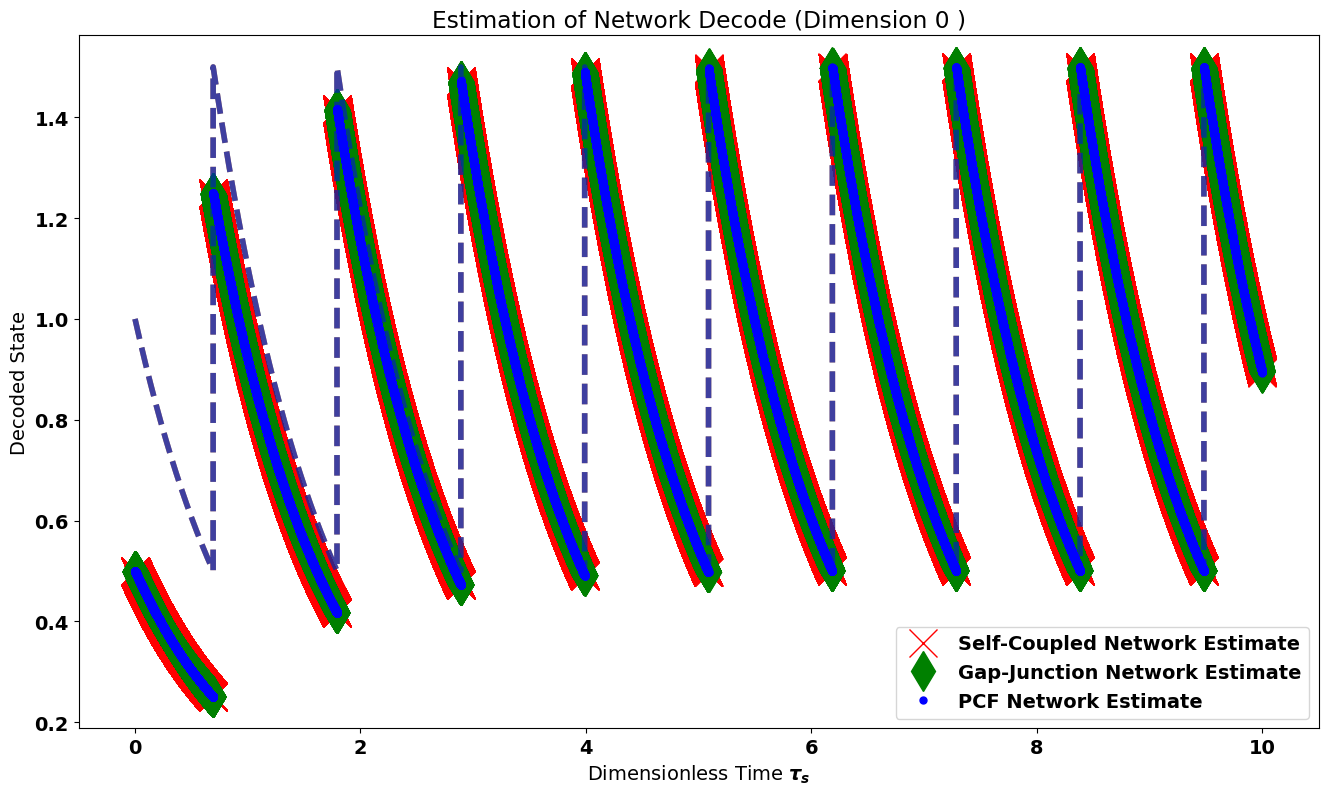
\includegraphics[width=\linewidth]{figures/const_dynamics_network_decode_comparison_sc_pcf_gj}
\caption{Simulation of self-coupled, gap-junction, and PCF networks. Network readouts for each are plotted. The dotted line is the derived expression(s) given by equations (\ref{eq:analysis:constant_driving_constant_dynamics_estimate_equation_explicit}) and (\ref{eq:analysis:comparison_sc_vs_pcf_vs_gj:const_dynamics:pcf_network_estimate_steady_state}). Note that all three trajectories are identical.}
\label{fig:analysis:comparison_sc_vs_pcf_vs_gj:network_decode_sc_pcf_gj}
\end{figure}

Next we plot the per-spike RMSE of each model for the same parameters while varying the spike rate. Figure (\ref{fig:analysis:comparison_sc_vs_pcf_vs_gj:per_spike_rmse_sc_pcf_gj}) shows the numerically measured per-spike RMSE for each model and their derived expressions, equations (\ref{eq:analysis:const_dynamics_per_spike_rmse_phi}) and (\ref{eq:analysis:comparison_sc_vs_pcf_vs_gj:per_spike_rmse_pcf_gj}). As the firing rate approaches the simulation timestep, $10^4$, the curves deviate from the derived expression. 

\begin{figure}
\centering
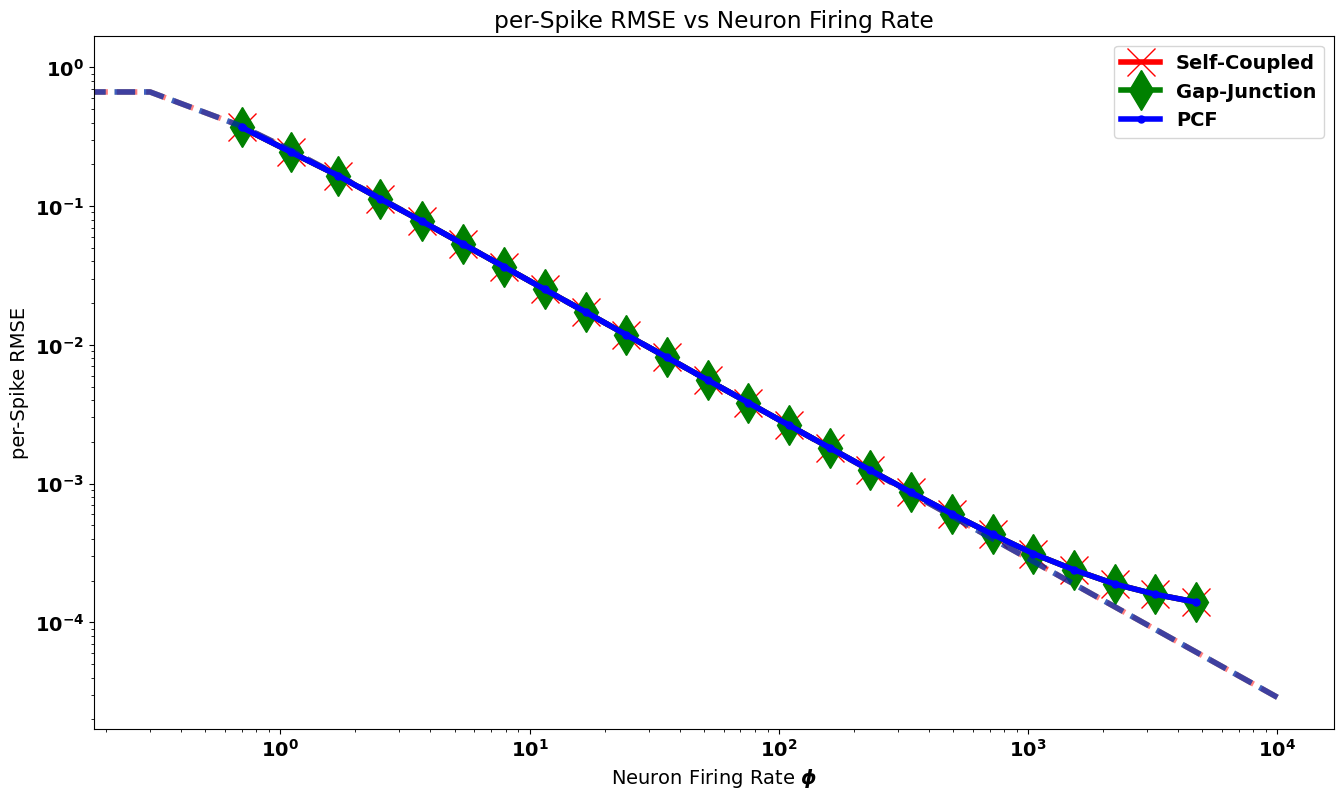
\includegraphics[width=\linewidth]{figures/per_spike_rmse_vs_phi_sc_gj_pcf}
\caption{Simulated per-spike RMSE for self-coupled, gap-junction, and PCF networks. The dotted lines are the derived expression for each model given by given by equations (\ref{eq:analysis:const_dynamics_per_spike_rmse_phi}) for the self-coupled and (\ref{eq:analysis:comparison_sc_vs_pcf_vs_gj:per_spike_rmse_pcf_gj}) for the gap-junction and PCF models respectively. Spike rates were estimated numerically by dividing the number of spikes by the simulation length. The RMSE was computed numerically by the discrete integral $\hat{RMSE} = \sqrt{\hat{\phi} \sum_{\tau \text{ between spikes }} e(\xi)^T e(\xi) \, \, d\xi }$. All computations used the numerically estimated spike rate.} 
\label{fig:analysis:comparison_sc_vs_pcf_vs_gj:per_spike_rmse_sc_pcf_gj}
\end{figure}

